\section{Estudo com Regressão Logística}

A \textbf{Regressão Logística} é um algoritmo que permite, estatisticamente e a partir dum conjuntos de observações de eventos passados, criar um modelo que possibilite a previsão de valores associados a um possível evento (caracterizado por um conjunto de variáveis).

Apesar de termos encontrado o trabalho apresentado na secção \ref{sec:bayes}, encontra-mos também outros trabalhos que se insidiam na catalogação de texto, mas que não utilizavam o \textit{dataset} que usámos. Um destes trabalhos foi um criado por um outro utilizador do \textit{Kaggle}, em que usava, entre outros algoritmos, \textbf{Regressão Logística} para catalogar o tema de noticias da \textit{BBC}. O seu estudo pode ser encontrado em \cite{kaggle_logistic}. Neste estudo é notado que foi atingida uma \textit{accuracy} para os dados de teste de $0.79$ para as 20 classes em estudo.

\subsection{Repartição dos dados}
A divisão dos dados neste estudo foi a mesma usada descrita na secção \ref{subsub:bayes_data}.


\subsection{Resultados obtidos}

Tal como na secção \ref{sub:results_bayes}, começamos por adaptar o código do autor original. Neste caso, sendo que ele possuía vários algoritmos para realizar o seu estudo, foi necessário filtrar só o código correspondente ao estudo de \textit{Regressão Logística}. Tal como no estudo das Redes de Bayes, neste caso usamos também a técnica de extracção de \textit{features} explicada na secção \ref{subsub:data_pre_processing} ao invés da usada pelo autor.

Ao fazermos o estudo da variação do hiperparâmetro C \footnote{Parâmetro de regularização. Quanto maior o seu valor, maior será a \textit{regularization strength}}, para 5000 iterações com \textit{early stopping}, obtivemos a variação de \textit{accuracy} apresentada no gráfico da figura \ref{diagram:accuracy_c_logistic}. Com este gráfico pode-se concluir que o maior valor da \textit{accuracy} para os dados de \textit{cross validation} foi obtido para um valor de $C = 10^{4}$.

\begin{figure}[t]
\begin{center}
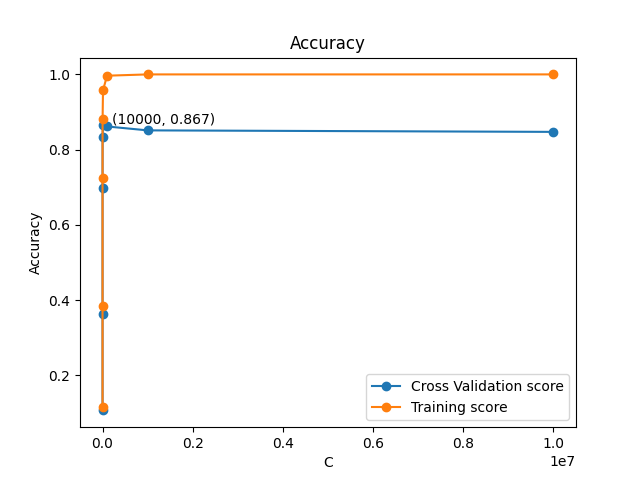
\includegraphics[width=0.5\textwidth,keepaspectratio]{figures/accuracy_C.png}
\caption{Gráfico da variação da \textit{accuracy} para valores de C entre $10^{0}$ e $10^{7}$, para os dados de treino e de \textit{cross validation}}
\label{diagram:accuracy_c_logistic}
\centering
\end{center}
\end{figure}

Desta forma, o nosso passo seguinte foi retreinar o melhor modelo obtido ($C = 10^{4}$) com os dados usados previamente para treino e \textit{cross validation}. As métricas de performance obtidas quando submetido o modelo final aos dados de teste podem ser consultadas na tabela \ref{tab:logistic_perforamnce}.

\begin{table}[!t]
\caption{Métricas de performance para $C = 10^{4}$}
\begin{center}
\begin{tabular}{l c c c c}
Class & Accuracy & Recall & Precision & F1 Score\\ \hline
0 & 0.9 & 0.9 & 0.893 & 0.998\\
1 & 0.805 & 0.805 & 0.957 & 0.895\\
2 & 0.85 & 0.85 & 0.949 & 0.902\\
3 & 0.9 & 0.9 & 0.965 & 0.954\\
4 & 0.795 & 0.795 & 0.909 & 0.858\\
5 & 0.91 & 0.91 & 0.917 & 0.92\\
6 & 0.895 & 0.895 & 0.986 & 0.929\\
7 & 0.91 & 0.91 & 0.964 & 0.993\\
8 & 0.815 & 0.815 & 0.868 & 0.829\\
9 & 0.95 & 0.95 & 0.996 & 0.983\\
10 & 0.785 & 0.785 & 0.943 & 0.901\\
11 & 0.935 & 0.935 & 0.985 & 0.976\\
12 & 0.815 & 0.815 & 0.925 & 0.997\\
13 & 0.94 & 0.94 & 0.985 & 0.961\\
14 & 0.835 & 0.835 & 0.85 & 0.879\\
15 & 0.865 & 0.865 & 0.957 & 0.943\\
16 & 0.96 & 0.96 & 0.988 & 0.992\\
17 & 0.91 & 0.91 & 0.987 & 0.991\\
18 & 0.855 & 0.855 & 0.991 & 0.891\\
19 & 0.875 & 0.875 & 0.967 & 0.911\\
20 & 0.895 & 0.895 & 0.955 & 0.897\\
21 & 0.96 & 0.96 & 0.944 & 0.941\\
22 & 0.845 & 0.845 & 0.8 & 0.947\\
23 & 0.775 & 0.775 & 0.928 & 0.764\\
24 & 0.955 & 0.955 & 0.992 & 0.999\\
25 & 0.73 & 0.73 & 0.896 & 0.885\\
26 & 0.87 & 0.87 & 0.911 & 0.925\\
27 & 0.96 & 0.96 & 0.995 & 0.983\\
28 & 0.935 & 0.935 & 0.897 & 0.968\\
29 & 0.845 & 0.845 & 0.868 & 0.942\\
30 & 0.82 & 0.82 & 0.983 & 0.969\\
31 & 0.875 & 0.875 & 0.933 & 0.889\\
32 & 0.91 & 0.91 & 0.98 & 0.983\\
33 & 0.84 & 0.84 & 0.92 & 0.972\\
34 & 0.85 & 0.85 & 0.946 & 0.837\\
35 & 0.955 & 0.955 & 0.981 & 0.986\\
36 & 0.905 & 0.905 & 0.872 & 0.87\\
37 & 0.89 & 0.89 & 0.918 & 0.987\\
38 & 0.87 & 0.87 & 0.954 & 0.884\\
39 & 0.89 & 0.89 & 0.92 & 0.998\\
40 & 0.905 & 0.905 & 0.896 & 0.921\\
41 & 0.745 & 0.745 & 0.892 & 0.837\\
42 & 0.835 & 0.835 & 0.98 & 0.896\\
43 & 0.9 & 0.9 & 0.977 & 0.949\\
44 & 0.88 & 0.88 & 0.986 & 0.899\\
45 & 0.945 & 0.945 & 0.989 & 0.964\\
46 & 0.835 & 0.835 & 0.974 & 0.957\\
47 & 0.915 & 0.915 & 0.959 & 0.941\\
48 & 0.865 & 0.865 & 0.932 & 0.984\\
49 & 0.905 & 0.905 & 0.985 & 0.978\\
\hline
Macro Average & 0.876 & 0.876 & 0.943 & 0.933\\
\end{tabular}
\label{tab:logistic_perforamnce}
\end{center}
\end{table}


\subsection{Conclusão}
Tal como na secção \ref{sec:bayes}, conseguimos neste exemplo obter uma performance melhor que a do autor do estudo original. Enquanto que este obteu uma \textit{accuracy} de teste de aproximadamente $0.79$ para apenas 20 classes, nós conseguimos obter uma \textit{accuracy} de aproximadamente $0.876$.
